% ==============================================================================
% Modelo para Especificação de Projeto de Software
% Prof. Vítor E. Silva Souza - NEMO/UFES :: DI/UFES :: PPGI/UFES
%
% Baseado em abtex2-modelo-trabalho-academico.tex, v-1.9.2 laurocesar
% Copyright 2012-2014 by abnTeX2 group at http://abntex2.googlecode.com/ 
%
% This work may be distributed and/or modified under the conditions of the LaTeX 
% Project Public License, either version 1.3 of this license or (at your option) 
% any later version. The latest version of this license is in
% http://www.latex-project.org/lppl.txt.
%
% IMPORTANTE:
% Instruções encontram-se espalhadas pelo documento. Para facilitar sua leitura,
% tais instruções são precedidas por (*) -- utilize a função localizar do seu
% editor para passar por todas elas.
% ==============================================================================

% Usa o estilo abntex2, configurando detalhes de formatação e hifenização.
\documentclass[
	12pt,				
	oneside,		
	a4paper,			
	english,			% Idioma adicional para hifenização.
	french,				% Idioma adicional para hifenização.
	spanish,			% Idioma adicional para hifenização.
	brazil				% O último idioma é o principal do documento.
	]{abntex2}


%%% Importação de pacotes. %%%

% Conserta o erro "No room for a new \count". 
% O comando \reserveinserts deve ser comentado ou não, dependendo da versão do LaTeX.
\usepackage{etex}
%\reserveinserts{28}

% Usa a fonte Latin Modern.
\usepackage{lmodern}

% Seleção de códigos de fonte.
\usepackage[T1]{fontenc}

% Codificação do documento em Unicode.
\usepackage[utf8]{inputenc}

% Usado pela ficha catalográfica.
\usepackage{lastpage}

% Indenta o primeiro parágrafo de cada seção.
\usepackage{indentfirst}

% Controle das cores.
\usepackage[usenames,dvipsnames]{xcolor}

% Inclusão de gráficos.
\usepackage{graphicx}

% Tabularx package: melhor controle de leiaute de tabelas.
\usepackage{tabularx}

% Inclusão de páginas em PDF diretamente no documento (para uso nos apêndices).
\usepackage{pdfpages}

% Para melhorias de justificação.
\usepackage{microtype}

% Citações padrão ABNT.
\usepackage[brazilian,hyperpageref]{backref}
\usepackage[alf]{abntex2cite}	
\renewcommand{\backrefpagesname}{Citado na(s) página(s):~}		% Usado sem a opção hyperpageref de backref.
\renewcommand{\backref}{}										% Texto padrão antes do número das páginas.
\renewcommand*{\backrefalt}[4]{									% Define os textos da citação.
	\ifcase #1
		Nenhuma citação no texto.
	\or
		Citado na página #2.
	\else
		Citado #1 vezes nas páginas #2.
	\fi}

% \rm is deprecated and should not be used in a LaTeX2e document
% http://tex.stackexchange.com/questions/151897/always-textrm-never-rm-a-counterexample
\renewcommand{\rm}{\textrm}

% Inclusão de símbolos não padrão.
\usepackage{amssymb}
\usepackage{eurosym}

% Para utilizar \eqref para referenciar equações.
\usepackage{amsmath}

% Permite mostrar figuras muito largas em modo paisagem com \begin{sidewaysfigure} ao invés de \begin{figure}.
\usepackage{rotating}

% Permite customizar listas enumeradas/com marcadores.
\usepackage{enumitem}

% Permite inserir hiperlinks com \url{}.
\usepackage{bigfoot}
\usepackage{hyperref}

% Permite usar o comando \hl{} para evidenciar texto com fundo amarelo. Útil para chamar atenção a itens a fazer.
\usepackage{soulutf8}

% Colorinlistoftodos package: to insert colored comments so authors can collaborate on the content.
% (*) Indicar o nome do aluno e substituir o nome do professor se for o caso.
\usepackage[colorinlistoftodos, textwidth=20mm, textsize=footnotesize]{todonotes}
\newcommand{\aluno}[1]{\todo[author=\textbf{Aluno},color=green!30,caption={},inline]{#1}}
\newcommand{\vitor}[1]{\todo[author=\textbf{Vítor},color=red!30,caption={},inline]{#1}}

% Permite inserir espaço em branco condicional (incluído no texto final só se necessário) em macros.
\usepackage{xspace}

% Permite incluir listagens de código com o comando \lstinputlisting{}.
\usepackage{listings}
\usepackage{caption}
\DeclareCaptionFont{white}{\color{white}}
\DeclareCaptionFormat{listing}{\colorbox{gray}{\parbox{\textwidth}{#1#2#3}}}
\captionsetup[lstlisting]{format=listing,labelfont=white,textfont=white}
\renewcommand{\lstlistingname}{Listagem}
\definecolor{mygray}{rgb}{0.5,0.5,0.5}
\lstset{
	basicstyle=\scriptsize,
	breaklines=true,
	numbers=left,
	numbersep=5pt,
	numberstyle=\tiny\color{mygray}, 
	rulecolor=\color{black},
	showstringspaces=false,
	tabsize=2,
    inputencoding=utf8,
    extendedchars=true,
    literate=%
    {é}{{\'{e}}}1
    {è}{{\`{e}}}1
    {ê}{{\^{e}}}1
    {ë}{{\¨{e}}}1
    {É}{{\'{E}}}1
    {Ê}{{\^{E}}}1
    {û}{{\^{u}}}1
    {ù}{{\`{u}}}1
    {â}{{\^{a}}}1
    {à}{{\`{a}}}1
    {á}{{\'{a}}}1
    {ã}{{\~{a}}}1
    {Á}{{\'{A}}}1
    {Â}{{\^{A}}}1
    {Ã}{{\~{A}}}1
    {ç}{{\c{c}}}1
    {Ç}{{\c{C}}}1
    {õ}{{\~{o}}}1
    {ó}{{\'{o}}}1
    {ô}{{\^{o}}}1
    {Õ}{{\~{O}}}1
    {Ó}{{\'{O}}}1
    {Ô}{{\^{O}}}1
    {î}{{\^{i}}}1
    {Î}{{\^{I}}}1
    {í}{{\'{i}}}1
    {Í}{{\~{Í}}}1
}




%%% Definição de variáveis. %%%
% (*) Substituir os textos abaixo com as informações apropriadas.
\titulo{SCMSS}
\autor{Gabriel Vila Real \and Luciano Coutinho Barcellos}
\local{Vitória, ES}
\data{2018}
\instituicao{
	Universidade Federal do Espírito Santo -- UFES
	\par
	Centro Tecnológico
	\par
	Departamento de Informática}
\newcommand{\subtitulo}{Documento de Projeto de Sistema}
\newcommand{\versao}{1.0}

% Define a capa.
% (*) Incluir linhas no registro de alterações a cada nova versão.
\renewcommand{\imprimircapa}{%
	\begin{capa}%
		\center
		
		{\ABNTEXchapterfont\large\subtitulo{}}
		\vfill
		\begin{center}
			\ABNTEXchapterfont\bfseries\LARGE\imprimirtitulo
		\end{center}
		
		\vfill
		Registro de Altera{\c c}{\~ o}es:
		\begin{table}[h]
			\centering
			\vspace{0.5cm}
			\begin{tabular}{|c|c|c|c|} \hline
			
 				Versão & Responsável & Data  & Alterações \\ \hline   
 				                            
				1.0  & \imprimirautor & 21/09/2018 & Versão Inicial  \\ \hline 
			\end{tabular}
		\end{table}
		
		\vfill
		\large\imprimirlocal
		\linebreak
		\large\imprimirdata
		\vspace*{1cm}
	\end{capa}
}

% Macros específicas do trabalho.
% (*) Inclua aqui termos que são utilizados muitas vezes e que demandam formatação especial.
% Exemplo: Java com TM (trademark) em superscript.
% Use sempre \xspace para que o LaTeX inclua espaço em branco após a macro somente quando necessário.
\newcommand{\java}{Java\texttrademark\xspace}




%%% Configurações finais de aparência. %%%

% Altera o aspecto de algumas cores.
\definecolor{blue}{RGB}{41,5,195}
\definecolor{lightgray}{gray}{0.9}

% Informações do PDF.
\makeatletter
\hypersetup{
	pdftitle={\@title}, 
	pdfauthor={\@author},
	pdfsubject={\imprimirpreambulo},
	pdfcreator={LaTeX with abnTeX2},
	pdfkeywords={abnt}{latex}{abntex}{abntex2}{trabalho acadêmico}, 
	colorlinks=true,				% Colore os links (ao invés de usar caixas).
	linkcolor=blue,					% Cor dos links.
	citecolor=blue,					% Cor dos links na bibliografia.
	filecolor=magenta,				% Cor dos links de arquivo.
	urlcolor=blue,					% Cor das URLs.
	bookmarksdepth=4
}
\makeatother

% Espaçamentos entre linhas e parágrafos.
\setlength{\parindent}{1.3cm}
\setlength{\parskip}{0.2cm}



%%% Páginas iniciais do documento: capa, folha de rosto, ficha, resumo, tabelas, etc. %%%

% Compila o índice.
\makeindex

% Inicia o documento.
\begin{document}

% Retira espaço extra obsoleto entre as frases.
\frenchspacing

% Inclui o brasão da UFES.
\begin{figure}[h]
  \centering
  
\includegraphics[scale=0.055]{brasao.jpg}
  \label{ppts3}
\end{figure} 

% Capa do trabalho.
\imprimircapa





%%% Início da parte de conteúdo do documento. %%%
% Marca o início dos elementos textuais.
\textual

% Inclusão dos capítulos.
\begingroup
\let\clearpage\relax
% ==============================================================================
% Projeto de Sistema - Nome do Aluno
% Capítulo 1 - Introdução
% ==============================================================================
\chapter{Introdução}
\label{sec-intro}

Este documento apresenta o documento de projeto (\textit{design}) arquitetural do sistema~\imprimirtitulo. Este documento está organizado da seguinte forma: a Seção~\ref{sec-plataforma} apresenta a plataforma de software utilizada na implementação da ferramenta; a Seção~\ref{sec-arquitetura} apresenta o projeto da arquitetura de software e suas subseções explicam cada uma de suas camadas.

O sistema~\imprimirtitulo visa permitir o controle de matrículas nos cursos de pós-graduação \textit{stricto sensu} no âmbito de um departamento da UFES, oferecendo suporte ao cadastro de cursos e de ofertas de disciplinas, permitindo aos alunos acessar e realizar suas solicitações de realização ou ajuste de matrículas, e aos professores orientadores aprovarem ou rejeitarem as solicitações de matrícula dos alunos.


\vspace*{2cm}
\endgroup
% ==============================================================================
% Projeto de Sistema - Nome do Aluno
% Capítulo 2 - Plataforma de Desenvolvimento
% ==============================================================================
\chapter{Plataforma de Desenvolvimento}
\label{sec-plataforma}

%=======================================================================================================
%			Tabela de Plataforma de Desenvolvimento e Tecnologias Utilizadas
%=======================================================================================================

Na Tabela~\ref{tabela-plataforma} são listadas as tecnologias utilizadas no desenvolvimento da ferramenta, bem como o propósito de sua utilização.

\begin{table}[h]
	\centering	
	\vspace{0.5cm}
	\footnotesize
	\caption{Plataforma de Desenvolvimento e Tecnologias Utilizadas}	
	\label{tabela-plataforma}
	\begin{tabular}{|p{1.6cm}|c|p{5cm}|p{6.5cm}|}  \hline 
 		Tecnologia & Versão & Descrição & Propósito \\\hline 
 		
		Java EE & 7 & Conjunto de especificação de APIs e tecnologias, que são implementadas por programas servidores de aplicação. & Redução da complexidade do desenvolvimento, implantação e gerenciamento de aplicações Web a partir de seus componentes de infra-estrutura prontos para o uso. \\ \hline

		Java & 8 & Linguagem de programação orientada a objetos e independente de plataforma. & Escrita do código-fonte das classes que compõem o sistema. \\\hline
		
		JSF & 2.2.12 & API para a construção de interfaces de usuários baseada em componentes para aplicações Web & Criação das páginas Web e sua comunicação com as classes Java.  \\\hline  
		
		EJB & 4.0.9 & API para construção de componentes transacionais gerenciados por \textit{container}. & Implementação das regras de negócio em componentes distribuídos, transacionais, seguros e portáveis. \\\hline
		
		JPA & 2.1 & API para persistência de dados por meio de mapeamento objeto/relacional. & Persistência dos objetos de domínio sem necessidade de escrita dos comandos SQL. \\\hline
		
		CDI & 1.1 & API para injeção de dependências. & Integração das diferentes camadas da arquitetura. \\\hline
		
		Facelets & 2.0 &  API para definição de decoradores (\textit{templates}) integrada ao JSF. & Reutilização da estrutura visual comum às paginas, facilitando a manutenção do padrão visual do sistema. \\\hline
		
		PrimeFaces & 6.2 &  Conjunto de componentes visuais JSF \textit{open source}. & Reutilização de componentes visuais Web de alto nível. \\\hline
		
		MySQL Server & 8.0 & Sistema Gerenciador de Banco de Dados Relacional gratuito. & Armazenamento dos dados manipulados pela ferramenta. \\\hline
		
		WildFly & 13 & Servidor de Aplicações para Java EE. & Fornecimento de implementação das APIs citadas acima e hospedagem da aplicação Web, dando acesso aos usuários via HTTP. \\\hline
	\end{tabular}
\end{table}






%=======================================================================================================
%			Tabela de Softwares de Apoio ao Desenvolvimento do Projeto
%=======================================================================================================

\newpage
Na Tabela~\ref{tabela-software} vemos os softwares que apoiaram o desenvolvimento da documentação e do código fonte.

\begin{table}[h]
	\centering	
	\vspace{0.5cm}
	\caption{Softwares de Apoio ao Desenvolvimento do Projeto}	
	\label{tabela-software}
	\begin{minipage}{\textwidth}
    	\begin{tabular}{|p{3cm}|c|p{4.5cm}|p{5.5cm}|}  \hline 
    	
     		Tecnologia &
     		Versão &
     		Descrição & 
     		Propósito 
     		\\\hline 
     		 
    		FrameWeb Editor &
    		1.0 &
    		Ferramenta CASE do método FrameWeb. &
    		Criação dos modelos de Entidades, Aplicação, Persistência e Navegação.
    		\\\hline
    
    		OverLeaf v2\footnote{OverLeaf v2, Online LaTeX Editor \url{http://v2.overleaf.com}} &
    		set/18 &
    		Editor de \LaTeX{} online. &
    		Redação da documentação do sistema, sendo usado o \textit{template} \textit{abnTeX}.
    		    \footnote{Suíte LaTeX para padrão ABNT \url{http://www.abntex.net.br}} 
		    \\\hline    
    
    		Eclipse Java EE IDE for Web Developers &
    		4.8 &
    		Ambiente de desenvolvimento (IDE) com suporte ao desenvolvimento Java EE. &
    		Implementação, implantação e testes da aplicação Web Java EE. 
    		\\\hline 
    		
    		%Apache Maven & 3.5 & Ferramenta de gerência e construção de projetos de software. & Obtenção e integração das dependências do projeto. \\\hline
    	\end{tabular}
	\end{minipage}
\end{table}


%% Capítulo 3 excluído porque não foi realizado o levantamento de requisitos
% \chapter{Atributos de Qualidade e Táticas}
\label{sec-atributos}

Na Tabela~\ref{tabela-atributos} são listados os atributos de qualidade considerados neste projeto, com uma indicação se os mesmos são condutores da arquitetura ou não e as táticas a serem utilizadas para tratá-los.

\begin{table}[h]
	\centering	
	\vspace{0.5cm}
	\caption{Atributos de Qualidade e Táticas Utilizadas}	
	\label{tabela-atributos}
	\begin{tabular}{|p{3.5cm}|p{2cm}|p{1.9cm}|p{7cm}|}  \hline 
	
 		Categoria & Requisitos Não Funcionais & Condutor da Arquitetura & Tática \\\hline 
 		
	\end{tabular}
\end{table}


\chapter{Arquitetura de Software}
\label{sec-arquitetura}

A arquitetura de software do sistema~\imprimirtitulo  segue a arquitetura padrão sugerida pelo FrameWeb~\cite{souza:masterthesis07,souza-et-al:iism09} baseada no padrão Camada de Serviço~\cite{fowler:book02}. A Figura~\ref{figura-arquitetura-padrao} ilustra a arquitetura e indica onde atuam os \textit{frameworks} para o desenvolvimento Web, listados na Tabela~\ref{tabela-plataforma}.

\begin{figure}[h]
	\centering
	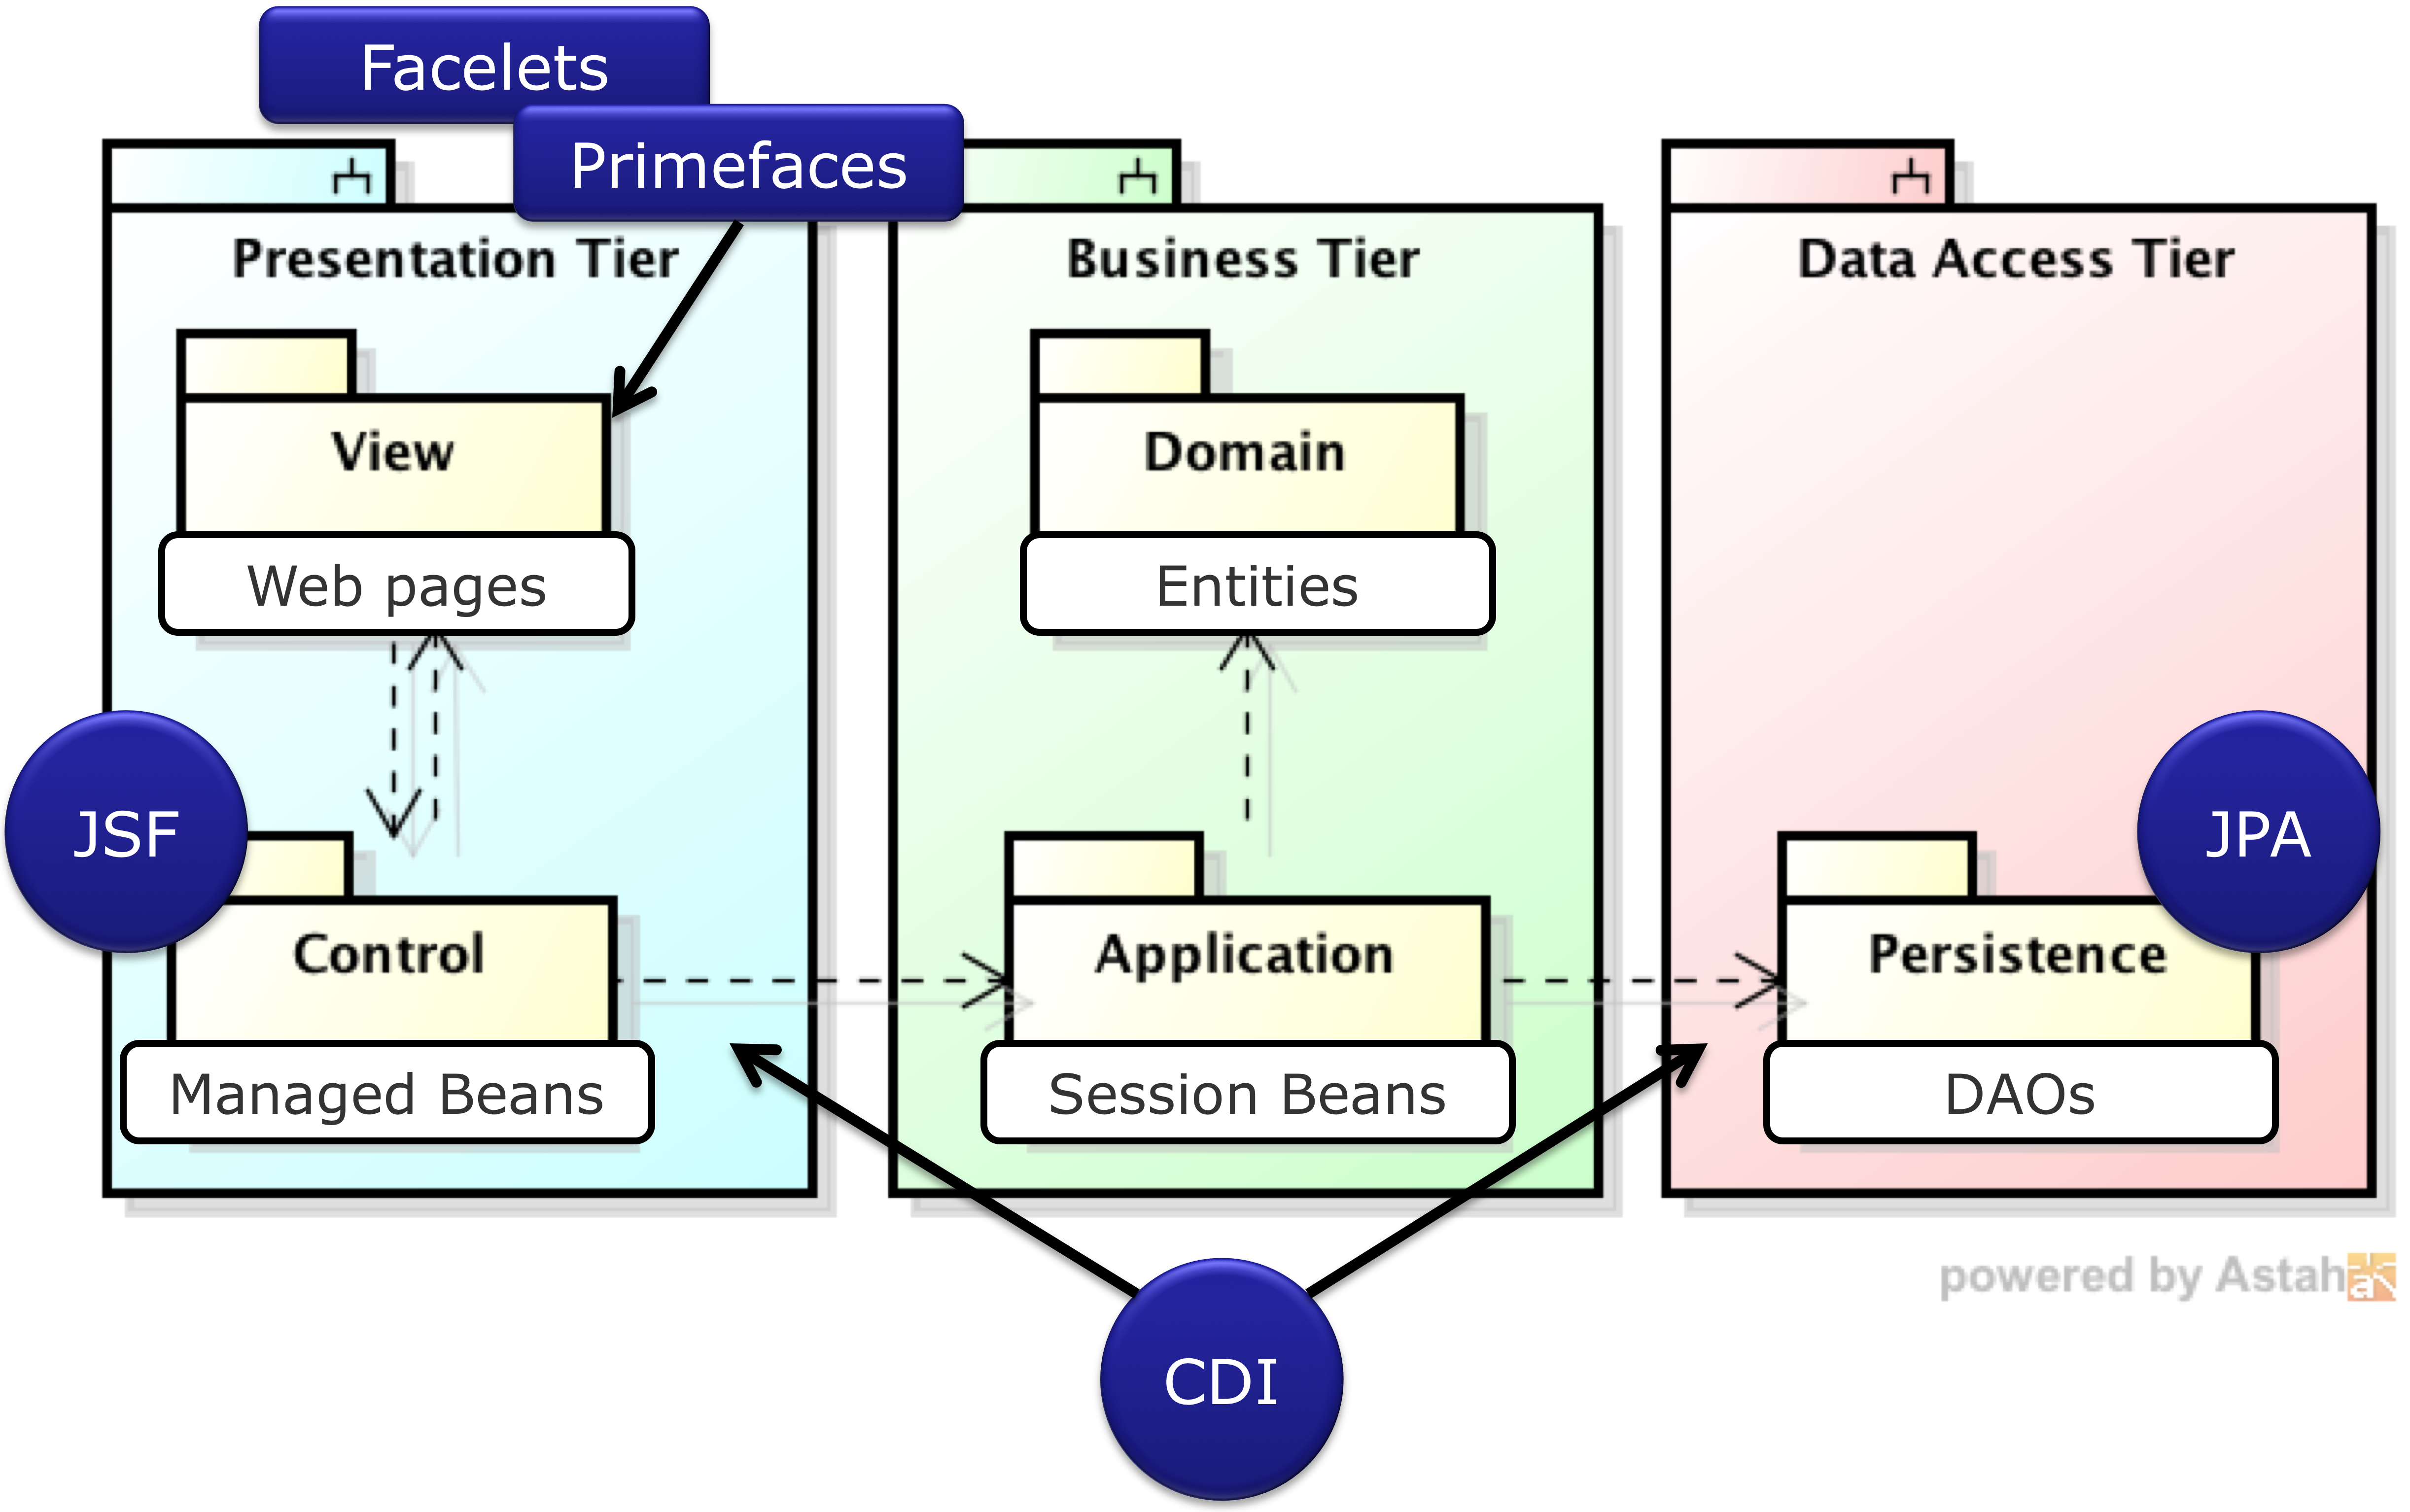
\includegraphics[width=0.8\textwidth]{figuras/figura-arquitetura-padrao.png}
	\caption{Arquitetura padrão proposta pelo FrameWeb.}
	\label{figura-arquitetura-padrao}
\end{figure}

Nas próximas seções, serão apresentados diagramas FrameWeb relativos a cada uma das camadas da arquitetura do sistema.

Alguns desses diagramas possuem algumas inconsistências decorrentes de pequenos problemas na ferramenta de edição utilizada.

\begin{itemize}

\item Uma das inconsistências trata-se dos tipos de dados genéricos nos atributos e nos métodos presentes nos diagramas. Não é possível na versão atual especificar o tipo de objeto presente nas coleções. \footnote{\url{https://github.com/nemo-ufes/FrameWeb/issues/5}}

\item Uma outra inconsistência se refere à cardinalidade em um relacionamento entre página e formulário. Não é possível especificar, na versão atual do editor, a cardinalidade de uma associação de navegação.\footnote{\url{https://github.com/nemo-ufes/FrameWeb/issues/6}}

\end{itemize}

Por fim, em alguns modelos de navegação, o controlador apresenta atributos que não são nem fornecidos como parâmetro a um dos métodos, nem obtidos do serviço. Estes casos devem-se a elementos não apresentados na presente versão deste documento, que não apresenta o sistema completo, mas apenas, visando cumprimento de prazos, apenas atende as exigências da atividade 1 de preparação do trabalho. A intenção é que alguns elementos como por exemplo \textit{aluno} no modelo de navegação de solicitação de matrícula, ou \textit{professor} no modelo de navegação de gerenciamento de solicitações de matrícula, estarão disponíveis na sessão do usuário, imediatamente após o \textit{login}.

\section{Camada de Apresentação}
\label{sec-arquitetura-apresentacao}



A Figura~\ref{navegacao-solicitar-matricula-10} mostra o modelo de navegação para a funcionalidade Solicitar Matrícula, que é realizada pelo aluno a partir do momento em que ele se encontra habilitado para cursar as disciplinas. Esta habilitação ocorre no momento em que uma pessoa (candidato) é aprovada na seleção, é aceita por um orientador a fim de iniciar no curso, e se comunica a secretaria do curso sobre o fato para a realização da matrícula no curso.

\begin{figure}[h]
	\centering
	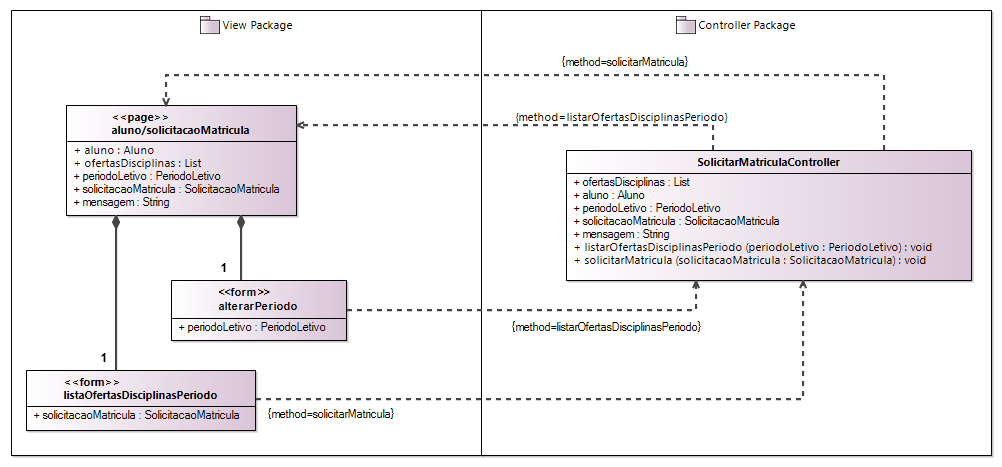
\includegraphics[width=0.8\textwidth]{figuras/navegacao-solicitar-matricula-10.png}
	\caption{Modelo de Navegação Solicitar Matrícula.}
	\label{navegacao-solicitar-matricula-10}
\end{figure}

A Figura~\ref{navegacao-gerenciar-solicitacoes-matricula-10} mostra o modelo de navegação para a funcionalidade onde o orientador avalia as solicitações de matrículas recebidas pelos alunos e fornece um parecer.

\begin{figure}[h]
	\centering
	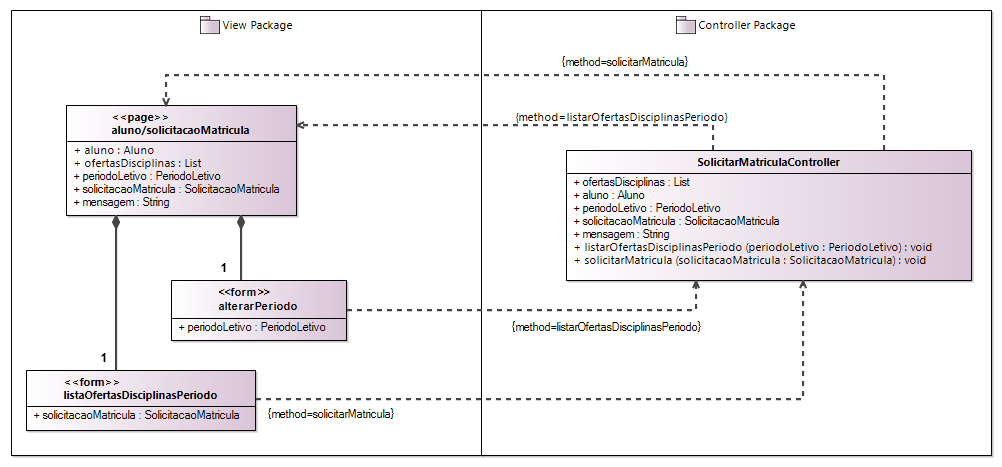
\includegraphics[width=0.8\textwidth]{figuras/navegacao-solicitar-matricula-10.png}
	\caption{Modelo de Navegação Gerenciar Solicitações de Matrícula.}
	\label{navegacao-gerenciar-solicitacoes-matricula-10}
\end{figure}

A Figura~\ref{navegacao-gerenciar-candidatos-10} mostra o modelo de navegação para as funcionalidades referentes ao cadastro dos candidatos aprovados no processo de seleção.

\begin{figure}[h]
	\centering
	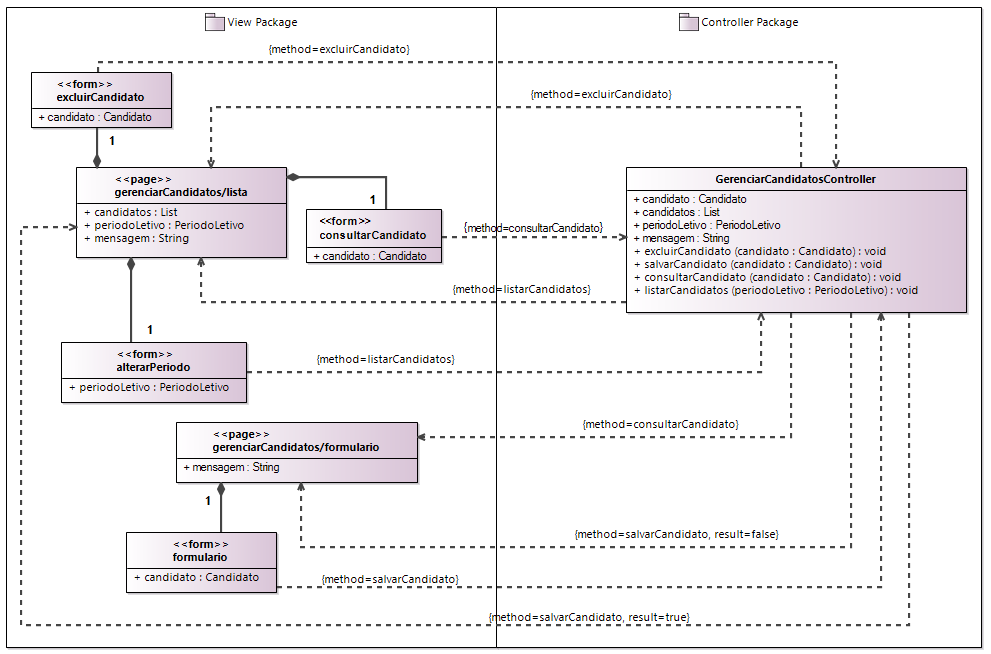
\includegraphics[width=0.8\textwidth]{figuras/navegacao-gerenciar-candidatos-10.png}
	\caption{Modelo de Navegação Gerenciar Candidatos.}
	\label{navegacao-gerenciar-candidatos-10}
\end{figure}



\section{Camada de Negócio}
\label{sec-arquitetura-negocio}

A Figura~\ref{modelo-entidades-10} exibe o modelo de entidades do sistema.

\begin{figure}[h]
	\centering
	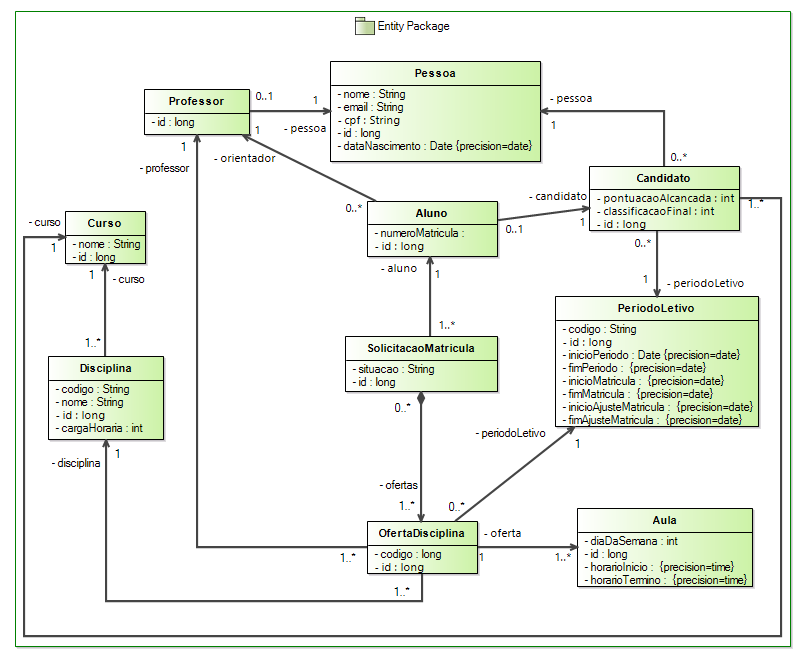
\includegraphics[width=0.8\textwidth]{figuras/modelo-entidades-10.png}
	\caption{Modelo de Entidades.}
	\label{modelo-entidades-10}
\end{figure}

A Figura~\ref{modelo-aplicacao-10} exibe o modelo de aplicação demonstrando as dependências entre os componentes da arquitetura.

\begin{figure}[h]
	\centering
	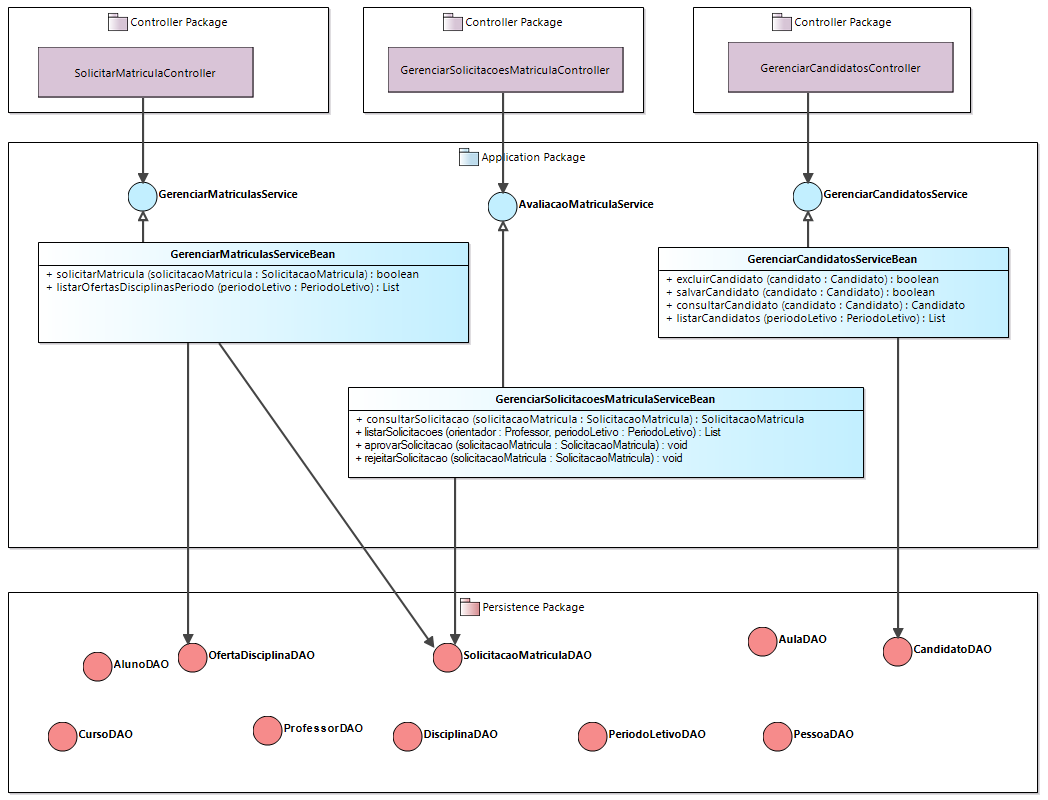
\includegraphics[width=0.8\textwidth]{figuras/modelo-aplicacao-10.png}
	\caption{Modelo de Aplicação.}
	\label{modelo-aplicacao-10}
\end{figure}

\section{Camada de Acesso a Dados}
\label{sec-arquitetura-dados}

A Figura~\ref{modelo-persistencia-10} exibe o modelo de persistência do sistema.

\begin{figure}[h]
	\centering
	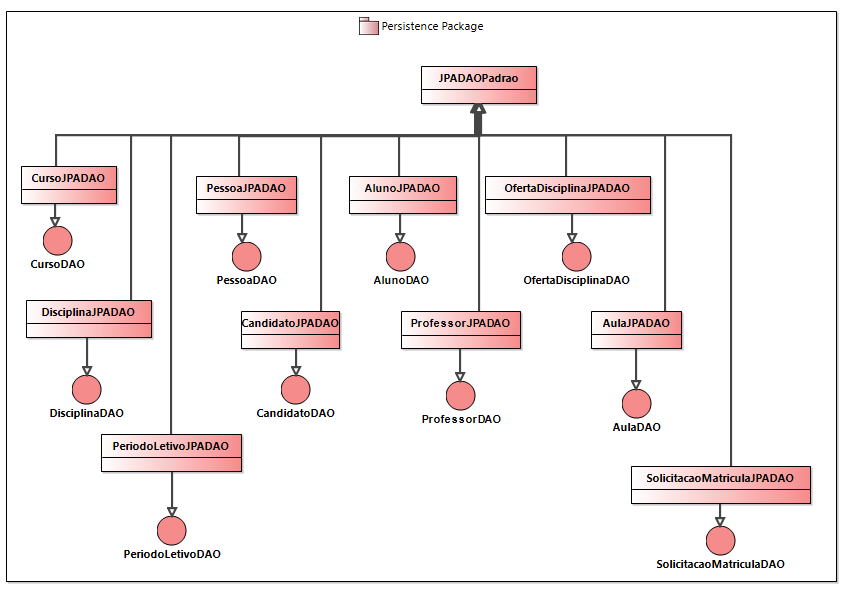
\includegraphics[width=0.8\textwidth]{figuras/modelo-persistencia-10.png}
	\caption{Modelo de Persistência}
	\label{modelo-persistencia-10}
\end{figure}






%%% Páginas finais do documento: bibliografia e anexos. %%%
% Finaliza a parte no bookmark do PDF para que se inicie o bookmark na raiz e adiciona espaço de parte no sumário.
\phantompart

% Marca o início dos elementos pós-textuais.
\postextual

% Referências bibliográficas
\bibliography{bibliografia}

% Índice remissivo.
\phantompart
\printindex

% Fim do documento.
\end{document}
